\documentclass{beamer}
\usetheme{metropolis}           % Use metropolis theme

\usepackage{graphicx}
\graphicspath{ {images/} }
\usepackage{adjustbox}
\usepackage{wrapfig}

\usepackage{multicol}

\title{Code Generation for Event-B}
\date{}
\author{Krikun Georgiy}
\institute{Innopolis University}

\begin{document}
  \maketitle

  \begin{frame}{Agenda}
    \tableofcontents
  \end{frame}

  \section{Formal Methods}

  \begin{frame}{Introduction Formal Methods}
    \textbf{Formal specification languages} are mathematically-based languages whose
    purpose is to aid the construction of systems and software. 

    % Rationale:

    % - higher quality of product\\
    % - reduce the cost of rework later on\\
    % - increase our understanding of a system\\
    % - eliminates ambiguity and reduces the chance of errors\\

    Roughly, formal design can be seen as a three step process:\\
    \begin{enumerate}
      \item Formal Specification
      \item Verification
      \item Implementation
    \end{enumerate}
    

  \end{frame}

  \begin{frame}{Introduction Formal Methods}
    \begin{columns}
      \column{0.3\textwidth}
        \textbf{Benefits:}\\
        - Discipline\\
        - Precision\\
      \column{0.6\textwidth}
        \textbf{Weaknesses:}\\
        - Expense\\
        - Limits Of Computational Models\\
        - Usability\\
    \end{columns}

    \end{frame}

    \begin{frame}{Formal Specification Languages}
      \textbf{Model-Based Languages:}\\
    Z, VDM, B

    \textbf{Finite State-Based Languages:}\\
    FSMs, SDL, Statecharts, X-machines

    \textbf{Process Algebra State-Based Languages:}\\
    CSP, CCS, LOTOS

    \textbf{Hybrid Languages:}\\
    CHARON
  \end{frame}

  \section{The B Method}
  
  \begin{frame}{The B Method}
    Developed by Jean-Raymond Abrial

    \textbf{Approach:}\\
    Starts from abstract model of a system\\
    Each refinement steps adds more details, provably consistent\\
    Obtain precise model which transform into an implementation


  \end{frame}

  \begin{frame}{The B Models}

    Use predicate calculus to model properties

    \textbf{B models are called machines} or Abstract Machines\\
    is given by:\\
    - \textbf{State} (variable set, state invariant) is the static part\\
    - a set of \textbf{Operations}, can modify the State, dynamic part

    For each operation must be proved that the specification preserves the
    invariant (Proof Obligation)

    Proof Obligations based on the Substitution Principle

  \end{frame}

  \section{The Event-B Methodology}

  \begin{frame}{The Event-B Methodology}

    Formal method is derived from the B method

    \textbf{Event-B models:}\\
    - machines (the dynamic part. e.g. variables, invariants, events)\\
    - contexts (the static part. e.g. carrier sets, constants)

    Basic relationships between machines and contexts:\\
    - a machine \textbf{sees} a context\\
    - a machine can \textbf{refine} another machine\\
    - a context can \textbf{extend} another context

  \end{frame}

  \begin{frame}{The Event-B Models}
    \centering
    \textbf{General structure}

    \begin{columns}
    \column{0.5\textwidth}
      \centering
      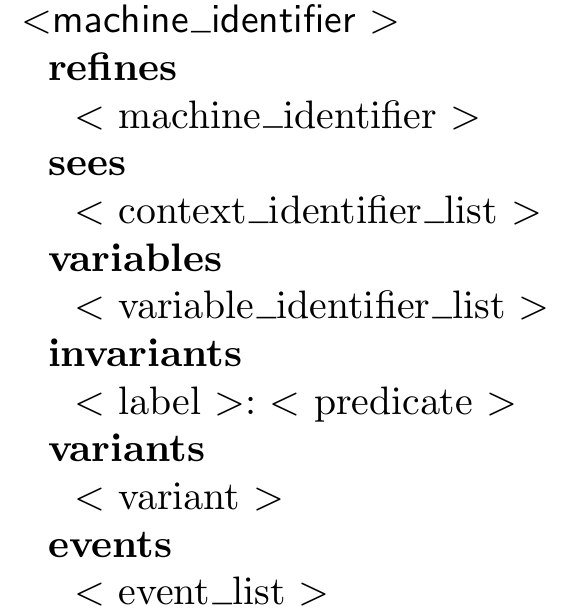
\includegraphics[width=\linewidth]{event-b_machine}
    \column{0.5\textwidth}
      \centering
      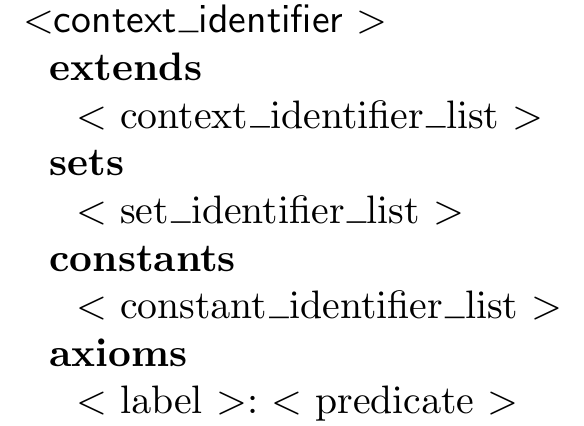
\includegraphics[width=\linewidth]{event-b_context}
    \end{columns}
  \end{frame}

  \section{Eiffel Programming Language + Design by Contract}

  \begin{frame}{Eiffel Programming Language}
    OOP language designed by Bertrand Meyer and Eiffel Software

    Structure of an Eiffel program:\\
    class $\rightarrow$ cluster $\rightarrow$ system $\rightarrow$ universe

    class - a set of features (attribute or routines)

    another classification - by role (commands and queries)

    \centering
    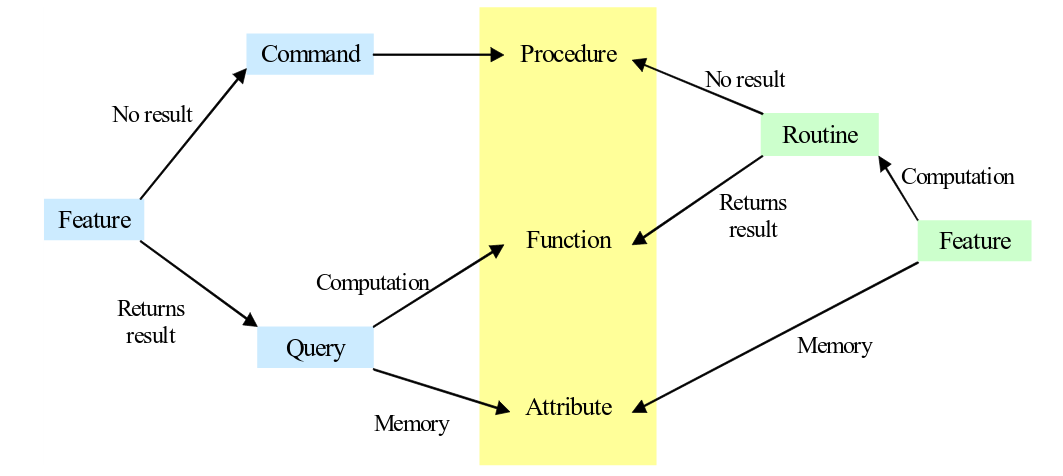
\includegraphics[width=0.8\linewidth]{eiffel_features}
    
  \end{frame}

  \begin{frame}{Design principles}

    Method principles:\\
    - Command/Query Separation Principle\\
    - Information Hiding\\
    - Uniform Access\\

  \end{frame}

  \begin{frame}{Design by Contract}
    \textbf{Design by Contract}
    is a method of software construction,
    which suggests building software
    systems that will cooperate on the basis
    of precisely defined contracts.\\[2em]

      Different kinds of contracts:\\
      - Preconditions\\
      - Postconditions\\
      - Class invariants\\
      - Check instructors\\
      - Loop invariants\\
      - Loop variants\\

  \end{frame}

  \begin{frame}{Design by Contract}

      \textbf{Benefits:}\\
      - Software correctness\\
      - Documentation\\
      - Debugging and testing\\
      - Management

  \end{frame}

  \section{Rodin (the Event-B IDE)}

  \begin{frame}{Rodin (the Event-B IDE)}
    The Rodin Platform is an Eclipse-based IDE for Event-B\\
    {\footnotesize \color{black!40}
      (The Rigorous Open Development Environment for Complex Systems)
    }

    provides a set of tools for Event-B models:\\
    - editor\\
    - proof generator\\
    - provers\\
    plugins provide extended functionality:\\
    - code generators\\
    - model checking\\
    - animation\\
    - visualization\\
    - etc

  \end{frame}

  \begin{frame}{Existing code generators}

    \textbf{EventB2Java}\\
    \textbf{EventB2JML}\\
    \textbf{EventB2Dafny}\\
    EventB2SQL\\
    EB2ALL \\
    B2C \\
    EHDL \\

  \end{frame}

  \section{Work plan until the end of the thesis}

  \begin{frame}{Work-plan}
    \begin{enumerate}
      \item Modeling code generator in Event-B as case study
      \item Generate code with EventB2Java
      \item Adapt code as plugin to Rodin
    \end{enumerate}
  \end{frame}

\end{document}